\documentclass{article}
\usepackage{tikz} 
\usepackage{import}
\usetikzlibrary{arrows,shapes.geometric,positioning}
\usepackage{color, colortbl}
\import{../../lib/latex/}{wgmlgz}
\begin{document}

\itmo[
  variant=161,
  labn=5,
  worktype=Домашняя работа,
  discipline=Дискретная математика,
  group=P3115,
  student=Владимир Мацюк,
  teacher=Поляков Владимир Иванович,
  logo=../../lib/img/itmo.png
]

Проверить на изоморфизм графы G1 и G2.

G1:
$$\begin{tabular}{|c|c|c|c|c|c|c|c|c|c|c|c|c|c|c|c|c|c|c|c|c|c|c|c|} \hline

    v/v & e1 & e2 & e3 & e4 & e5 & e6 & e7 & e8 & e9 & e10 & e11 & e12 \nl
    e1  &    & 3  &    &    & 4  & 4  & 4  & 4  &    & 3   & 4   & \nl
    e2  & 3  &    & 1  &    &    &    &    & 4  &    & 2   &     & \nl
    e3  &    & 1  &    & 5  &    &    &    &    & 3  & 1   &     & \nl
    e4  &    &    & 5  &    & 1  & 4  & 1  &    & 4  & 5   & 4   & \nl
    e5  & 4  &    &    & 1  &    & 1  &    &    &    & 3   &     & \nl
    e6  & 4  &    &    & 4  & 1  &    & 2  &    &    &     & 4   & \nl
    e7  & 4  &    &    & 1  &    & 2  &    &    &    & 4   &     & 1 \nl
    e8  & 4  & 4  &    &    &    &    &    &    & 3  & 3   &     & 5 \nl
    e9  &    &    & 3  & 4  &    &    &    & 3  &    &     & 5   & \nl
    e10 & 3  & 2  & 1  & 5  & 3  &    & 4  & 3  &    &     & 2   & \nl
    e11 & 4  &    &    & 4  &    & 4  &    &    & 8  & 2   &     & 4 \nl
    e12 &    &    &    &    &    &    & 1  & 5  &    &     & 4   & \nl
  \end{tabular}$$

G2:
$$\begin{tabular}{|c|c|c|c|c|c|c|c|c|c|c|c|c|c|c|c|c|c|c|c|c|c|c|c|} \hline
    v/v & e1 & e2 & e3 & e4 & e5 & e6 & e7 & e8 & e9 & e10 & e11 & e12 \nl
    e1  &    &    &    &    & 4  &    &    & 1  &    & 4   & 2   & 4 \nl
    e2  &    &    &    & 1  &    & 2  & 4  &    &    & 3   &     & \nl
    e3  &    &    &    & 3  & 5  &    & 3  &    &    &     &     & 4 \nl
    e4  &    & 1  & 3  &    &    & 1  &    &    &    &     &     & 5 \nl
    e5  & 4  &    & 8  &    &    & 2  &    &    & 4  & 4   &     & 4 \nl
    e6  &    & 2  &    & 1  & 2  &    & 3  & 3  &    & 3   & 4   & 5 \nl
    e7  &    & 4  & 3  &    &    & 3  &    &    & 5  & 4   &     & \nl
    e8  & 1  &    &    &    &    & 3  &    &    &    & 4   &     & 1 \nl
    e9  &    &    &    &    & 4  &    & 5  &    &    &     & 1   & \nl
    e10 & 4  & 3  &    &    & 4  & 3  & 4  & 4  &    &     & 4   & \nl
    e11 & 2  &    &    &    &    & 4  &    &    & 1  & 4   &     & 1  \nl
    e12 & 4  &    & 4  & 5  & 4  & 5  &    & 1  &    &     & 1   & \nl
  \end{tabular}$$


Для графа G1     Σρ(x)=62. Список Ρ(x) = {8, 7, 7, 6, 5, 5, 5, 4, 4, 4, 4, 3}.

Для графа G2     Σρ(y)=62. Список Ρ(y) = {8, 7, 7, 6, 5, 5, 5, 4, 4, 4, 4, 3}.

Разобьем вершины обоих графов на классы по их степеням.


\definecolor{Green}{rgb}{0.5,1,0.2}
$$\begin{tabular}{|c|c|c|c|c|c|c|c|c|c|c|c|c|c|c|c|c|c|c|c|c|c|c|c|} \hline
      & p(x) = p(y) = 8 & p(x) = p(y) = 7 & p(x) = p(y) = 6 & p(x) = p(y) = 5 & p(x) = p(y) = 4 & p(x) = p(y) = 3 \nl
    X & x10             & x1 x4           & x11             & x6 x7 x8        & x2 x3 x5 x9     & x12\nl
    Y & y6              & y10 y12         & y5              & y1 y7 y11       & y2 y3 y4 y8     & y9 \nl
  \end{tabular}$$
Из таблицы сразу видно соответствие вершин графов
$$\begin{tabular}{|c|c|c|c|c|c|c|c|c|c|c|c|c|c|c|c|c|c|c|c|c|c|c|c|} \hline
    X   & Y \nl
    \rowcolor{Green}
    x10 & y6\nl
    \rowcolor{Green}
    x11 & y5\nl
    \rowcolor{Green}
    x12 & y9\nl
  \end{tabular}$$


Для определения соответствия вершин с ρ(x) = ρ(y) = 5 попробуем связать с установленными вершинами из ρ(x) = ρ(y) = 8 и ρ(x) = ρ(y) = 6 и ρ(x) = ρ(y) = 3.
    
    $$\begin{tabular}{|c|c|c|c|c|c|c|c|} \hline X & Y \nl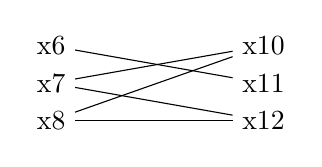
\begin{tikzpicture}[ -, node distance = 1cm, 
                    auto, main/.style = {}]\begin{scope}[node distance=0mm and 20mm]
    \node[main] (10)  {x10};
\node[main, below= of 10] (11)  {x11};
\node[main, below= of 11] (12)  {x12};
\node[main, left= of 10] (6)  {x6};
\node[main, below= of 6] (7)  {x7};
\node[main, below= of 7] (8)  {x8};
    \path[every node/.style={sloped,anchor=south,auto=false}]
(10) edge (7)
(10) edge (8)
(11) edge (6)
(12) edge (7)
(12) edge (8);\end{scope}  \end{tikzpicture} &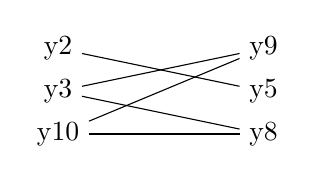
\begin{tikzpicture}[ -, node distance = 1cm, 
                    auto, main/.style = {}]\begin{scope}[node distance=0mm and 20mm]
    \node[main] (9)  {y9};
\node[main, below= of 9] (5)  {y5};
\node[main, below= of 5] (8)  {y8};
\node[main, left= of 9] (2)  {y2};
\node[main, below= of 2] (3)  {y3};
\node[main, below= of 3] (10)  {y10};
    \path[every node/.style={sloped,anchor=south,auto=false}]
(5) edge (2)
(8) edge (3)
(8) edge (10)
(9) edge (3)
(9) edge (10);\end{scope}  \end{tikzpicture}   \nl \end{tabular}$$Анализ связей показывает следующее соответствие:
    $$\begin{tabular}{|c|c|c|c|c|c|c|c|} \hline X & Y \nl\rowcolor{Green} x6 & y5\nl 
\rowcolor{Green} x7 & y1\nl 
\rowcolor{Green} x8 & y12\nl 
 x10 & y7\nl 
 x11 & y2\nl 
 x12 & y3\nl   \end{tabular}$$
    
    Для определения соответствия вершин с ρ(x) = ρ(y) = 7 попробуем связать с установленными вершинами из ρ(x) = ρ(y) = 8 и ρ(x) = ρ(y) = 6 и ρ(x) = ρ(y) = 3 и ρ(x) = ρ(y) = 5.
    
    $$\begin{tabular}{|c|c|c|c|c|c|c|c|} \hline X & Y \nl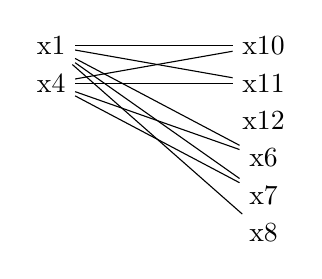
\begin{tikzpicture}[ -, node distance = 1cm, 
                    auto, main/.style = {}]\begin{scope}[node distance=0mm and 20mm]
    \node[main] (10)  {x10};
\node[main, below= of 10] (11)  {x11};
\node[main, below= of 11] (12)  {x12};
\node[main, below= of 12] (6)  {x6};
\node[main, below= of 6] (7)  {x7};
\node[main, below= of 7] (8)  {x8};
\node[main, left= of 10] (1)  {x1};
\node[main, below= of 1] (4)  {x4};
    \path[every node/.style={sloped,anchor=south,auto=false}]
(6) edge (1)
(6) edge (4)
(7) edge (1)
(7) edge (4)
(8) edge (1)
(10) edge (1)
(10) edge (4)
(11) edge (1)
(11) edge (4);\end{scope}  \end{tikzpicture} &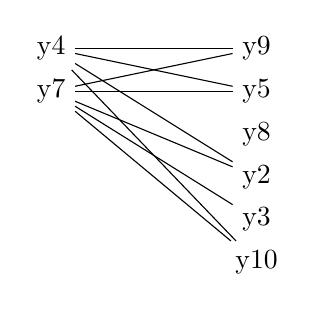
\begin{tikzpicture}[ -, node distance = 1cm, 
                    auto, main/.style = {}]\begin{scope}[node distance=0mm and 20mm]
    \node[main] (9)  {y9};
\node[main, below= of 9] (5)  {y5};
\node[main, below= of 5] (8)  {y8};
\node[main, below= of 8] (2)  {y2};
\node[main, below= of 2] (3)  {y3};
\node[main, below= of 3] (10)  {y10};
\node[main, left= of 9] (4)  {y4};
\node[main, below= of 4] (7)  {y7};
    \path[every node/.style={sloped,anchor=south,auto=false}]
(2) edge (4)
(2) edge (7)
(3) edge (7)
(5) edge (4)
(5) edge (7)
(9) edge (4)
(9) edge (7)
(10) edge (4)
(10) edge (7);\end{scope}  \end{tikzpicture}   \nl \end{tabular}$$Анализ связей показывает следующее соответствие:
    $$\begin{tabular}{|c|c|c|c|c|c|c|c|} \hline X & Y \nl\rowcolor{Green} x1 & y9\nl 
\rowcolor{Green} x4 & y4\nl 
 x6 & y5\nl 
 x7 & y1\nl 
 x8 & y12\nl 
 x10 & y7\nl 
 x11 & y2\nl 
 x12 & y3\nl   \end{tabular}$$
    
    Для определения соответствия вершин с ρ(x) = ρ(y) = 4 попробуем связать с установленными вершинами из ρ(x) = ρ(y) = 8 и ρ(x) = ρ(y) = 6 и ρ(x) = ρ(y) = 3 и ρ(x) = ρ(y) = 5 и ρ(x) = ρ(y) = 7.
    
    $$\begin{tabular}{|c|c|c|c|c|c|c|c|} \hline X & Y \nl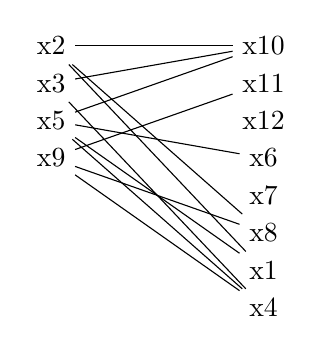
\begin{tikzpicture}[ -, node distance = 1cm, 
                    auto, main/.style = {}]\begin{scope}[node distance=0mm and 20mm]
    \node[main] (10)  {x10};
\node[main, below= of 10] (11)  {x11};
\node[main, below= of 11] (12)  {x12};
\node[main, below= of 12] (6)  {x6};
\node[main, below= of 6] (7)  {x7};
\node[main, below= of 7] (8)  {x8};
\node[main, below= of 8] (1)  {x1};
\node[main, below= of 1] (4)  {x4};
\node[main, left= of 10] (2)  {x2};
\node[main, below= of 2] (3)  {x3};
\node[main, below= of 3] (5)  {x5};
\node[main, below= of 5] (9)  {x9};
    \path[every node/.style={sloped,anchor=south,auto=false}]
(1) edge (2)
(1) edge (5)
(4) edge (3)
(4) edge (5)
(4) edge (9)
(6) edge (5)
(8) edge (2)
(8) edge (9)
(10) edge (2)
(10) edge (3)
(10) edge (5)
(11) edge (9);\end{scope}  \end{tikzpicture} &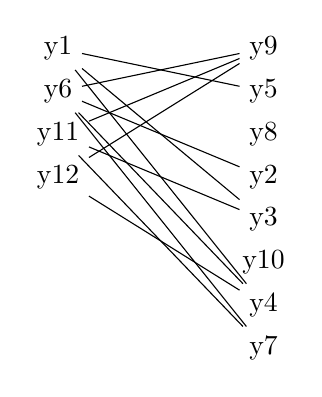
\begin{tikzpicture}[ -, node distance = 1cm, 
                    auto, main/.style = {}]\begin{scope}[node distance=0mm and 20mm]
    \node[main] (9)  {y9};
\node[main, below= of 9] (5)  {y5};
\node[main, below= of 5] (8)  {y8};
\node[main, below= of 8] (2)  {y2};
\node[main, below= of 2] (3)  {y3};
\node[main, below= of 3] (10)  {y10};
\node[main, below= of 10] (4)  {y4};
\node[main, below= of 4] (7)  {y7};
\node[main, left= of 9] (1)  {y1};
\node[main, below= of 1] (6)  {y6};
\node[main, below= of 6] (11)  {y11};
\node[main, below= of 11] (12)  {y12};
    \path[every node/.style={sloped,anchor=south,auto=false}]
(2) edge (6)
(3) edge (1)
(3) edge (11)
(4) edge (1)
(4) edge (6)
(4) edge (12)
(5) edge (1)
(7) edge (6)
(7) edge (11)
(9) edge (6)
(9) edge (11)
(9) edge (12);\end{scope}  \end{tikzpicture}   \nl \end{tabular}$$Анализ связей показывает следующее соответствие:
    $$\begin{tabular}{|c|c|c|c|c|c|c|c|} \hline X & Y \nl x1 & y9\nl 
\rowcolor{Green} x2 & y6\nl 
\rowcolor{Green} x3 & y8\nl 
 x4 & y4\nl 
\rowcolor{Green} x5 & y11\nl 
 x6 & y5\nl 
 x7 & y1\nl 
 x8 & y12\nl 
\rowcolor{Green} x9 & y10\nl 
 x10 & y7\nl 
 x11 & y2\nl 
 x12 & y3\nl   \end{tabular}$$
    
    

По итоговой таблице связей можно сделать вывод, что каждой вершине графа G1 соответствует одна вершина графа G2, что доказывает изоморфизм данных графов.



\end{document}